% !TeX root = ..\academicWriting.tex SHOULD WORK BUT DOESN'T :(

% Notes for titlepage
\note{Hi everybody welcome to this course! Here we'll put into practice the concepts learnt in the previous theory sessions using LaTeX to produce academic documents.}

\begin{frame}{What's LaTeX?}
 \begin{fullpageitemize}
  \itemR Markup language
  \itemR High quality documents
  \itemR Consistent output every time
  \itemR Separation of style from text
  \itemR Easy academic format: equations, glossaries, bibliography, table of contents, cross references\ldots
 \end{fullpageitemize}
 \note{LaTeX is a markup language aiming to produce high quality documents. It was created by academics, with the idea of having consistent output every time (forget that table that moved itself from page 2 to 5), separation of style from text (that has two objetives: helps centre oneself in the content and allows the reuse of material) and easy academic format (equations are not a pain, glossaries, bibliographies and tables of contents automatic and cross referencing trivial)
 
So let's see how can we start using the stuff. As a note I'll talk mostly about free software because that's what I use}
\end{frame}

\begin{frame}{What do I need?}
 \null{\color{colororange}\largetext{Option 1}}
 \begin{itemize}
  \item \textbf{Editor}: general purpose or specific (\href{http://www.xm1math.net/texmaker/}{Texmaker}, \href{https://www.tug.org/texworks/}{TeXworks}, \href{https://kile.sourceforge.io/}{Kile})
  
  \item \textbf{Distribution}: \href{https://miktex.org/}{MikTeX} (Windows), \href{https://tug.org/texlive/}{TeXLive} (cross-platform) $\rightarrow$ compiler + packages
 \end{itemize}
 \vspace{1ex}
 {\color{colororange}\largetext{Option 2}}
  \begin{itemize}
  \item \textbf{Online editor}: \href{https://www.overleaf.com/}{Overleaf}
 \end{itemize}
 
 \note{We're going to write in plain text so any editor can do. I use Emacs (in general I write in Org mode and export to LaTeX). Also the AucTeX mode is specially useful. For starters, and with the idea of not getting crazy, one can use a specific editor as Texmaker that I used to produce these slides.
 
 We also need a distribution of LaTeX. If you're on Windows I'd recommend MikTeX as it takes care of needed packages on its own. If you're on Linux you know you to deal with packages!
 
 The other option is using an online service as Overleaf that takes care of the process. I use it mostly for trying templates, so if you plan to take this way, I can't help!}
\end{frame}

\begin{frame}{The markup language}
 \begin{fullpageitemize}
  \itemR We use \textbf{labels} to \textbf{mark} the parts of the text we want to have a \textbf{specific style}
  \itemR After compilation, we obtain a \textbf{styled document}
  \itemR Documents must follow a concrete structure
  \itemR Specific syntax for equations, figures, tables, titles, sections\ldots
 \end{fullpageitemize}
 \note{So, how we write in this LaTeX stuff? Easy! We just \emph{mark} the parts of the text we want to have a specific format with some  \emph{labels} that LaTeX understands, then it'll \emph{compile} our doc and produce a styled output.
 
 For this to be possible our documents must follow a concrete structure and we have to use a specific syntax for defining elements as equations, figures, tables or titles.}
\end{frame}

\begin{frame}[fragile]{Structure of a document}
\null{\inconsolatafont .tex} files with the following structure:
 \begin{lstlisting}[language={[LaTeX]TeX},texcsstyle=*\color{colororange}]
   % Document definition   
   \documentclass[OPTIONS]{TYPE}
   %%%%%%% Preamble %%%%%%
   \usepackage{PACKAGE} 
   % Data
   \title{TITLE}
   \author{AUTHOR}   
   %%%%%%%%%%%%%%%%%%%%%%%%
   \begin{document}       
   % Body of document          
   \end{document}
 \end{lstlisting}
 
 \note{We write {\inconsolatafont .tex} files with a specific structure divided in two parts: the preamble, that goes from the definition of the document to the body and where we add packages, commands and data and after, the body of the document, where we write the contents.
 
 The cited packages are pieces of LaTeX that people wrote and give us added functionality as language support. They're centralised in a repository called \href{https://www.ctan.org/}{CTAN} and we have to install them to use them.}

\end{frame}

\begin{frame}[fragile]{Defining elements}
\vspace{2ex}
\textbf{Equations}
\begin{LTXexample}[pos=r,wide,width=.5,rframe={}, language={[LaTeX]TeX},texcsstyle=*\color{colororange}]
\begin{equation}
  A = \pi\times R^2
\end{equation}
\end{LTXexample}
\vspace{1ex}
\textbf{Figures}
\vspace{-1ex}
\begin{LTXexample}[pos=r,wide,width=.25,rframe={}, language={[LaTeX]TeX},texcsstyle=*\color{colororange}]
\begin{figure}[h] % h: here
  \centering
  \includegraphics
  [width=\textwidth] % options
  {images/manatee} % path
\end{figure}
\end{LTXexample}

\note{\footnotesize{Here you can see the syntax for introducing equations and figures. The equation has a number that can be avoided using the equation* environment. Also, we can have both inline equations that are written between dollar signs. There is a special syntax for typesetting equations that's a bit complex to get, an online editor or a good IDE can help a lot at the beginning.

Regarding figures, there are both inline and floating figures, the one shown is a floating one. We'll talk about floating elements after, but I'd like to point out a feature of all commands and environments: the options between brackets are optional and the ones between braces compulsory. So here, the path is of course compulsory. The extension can be omitted.}}
\end{frame}

\begin{frame}[fragile]{Defining elements}
\textbf{Tables}
\begin{LTXexample}[pos=r,wide,width=.3,rframe={}, language={[LaTeX]TeX},texcsstyle=*\color{colororange}]
\begin{table}
 \begin{tabular}{cc} % c: center
  \hline
  \textbf{A} & \textbf{B} \\ 
  \hline
  x          & 1          \\
  y          & 2          \\
  \hline
 \end{tabular}
\end{table}
\end{LTXexample}
\note{Here you can see an example of a table. Tables in LaTeX are a pain to write, so at the end I'm linking some tricks to alleviate the work. They can be as well floating elements or not and consist on some data separated by \& and backslashes}
\end{frame}

\begin{frame}[fragile]{Defining elements}
\textbf{Title, chapters, sections}
\begin{LTXexample}[pos=r,wide,width=.3,rframe={}, language={[LaTeX]TeX},texcsstyle=*\color{colororange}]

\end{LTXexample}
\note{}
\end{frame}

\begin{frame}[fragile]{Defining elements}
\textbf{Lists}
\begin{LTXexample}[pos=r,wide,width=.3,rframe={}, language={[LaTeX]TeX},texcsstyle=*\color{colororange}]

\end{LTXexample}
\note{}
\end{frame}

\begin{frame}{Crossreferences}

\note{If we add a label to any element, we can after reference it. We need to compile an additional time so as to get all the references. The editors let you choose (example in Texmaker)

label ref, paquete cleveref (cref, Cref), nameref}
\end{frame}

\begin{frame}{Captions}
\note{Floating elements as figures, tables and code listings can have captions. Caption is positioned where we asked it to be.}
\end{frame}

\begin{frame}{Bibliography}
 \begin{fullpageitemize}
  \itemR Bibliography stored in a {\inconsolatafont .bib} file 
  \itemR Managed by external program (\href{http://www.bibtex.org/}{BibTeX}, \ldots) 
  \itemR Additional compilation step: {\inconsolatafont latex - bibtex - latex - latex}
  \itemR Bibliography managers: JabRef, Zotero, \href{https://bibdesk.sourceforge.io/}{BibDesk} \ldots
 \end{fullpageitemize}
 
 \note{zotero-better-bibtex,  for Mac. 
 BibTeX comes with the standard LaTeX distribution, there are more options like Natbib, BibLaTeX}
\end{frame}

\begin{frame}[fragile]{Bibliography}

MWE with bibliography defined in {\inconsolatafont references.bib}:

\begin{lstlisting}[language={[LaTeX]TeX},texcsstyle=*\color{colororange}]
\documentclass[11pt]{article}
  \begin{document}
  
  As said in \cite{Knuth1997}...
    
  % Definition of bibliography
  \bibliography{references} % Path
  \bibliographystyle{plain} % Style
\end{document}
\end{lstlisting}

\note{Minimum working example}

\end{frame}

\begin{frame}[fragile]{Bibliography}

Where {\inconsolatafont references.bib} looks like:

\begin{lstlisting}[breaklines=false]
@book{Knuth1997,
  title={The art of computer programming},
  author={Knuth, Donald Ervin},
  volume={3},
  year={1997},
  publisher={Pearson Education}}
\end{lstlisting}
\note{A little trick is changing Scholar settings so that one can directly import to BibTex}
\end{frame}

\begin{frame}{Useful packages}

\end{frame}

\begin{frame}{Tools \& tricks}
 \begin{fullpageitemize}
  \itemR \href{https://www.overleaf.com/}{\textbf{Overleaf}}: templates and online editor
  \itemR \href{http://wiki.inkscape.org/wiki/index.php/LaTeX}{\textbf{Inkscape}}: image text as document text, LaTeX equation in images
  \itemR \href{https://www.ctan.org/tex-archive/support/excel2latex/}{\textbf{Excel2LaTeX}}: export tables with LaTeX format
  \itemR \href{http://detexify.kirelabs.org/classify.html}{\textbf{Detexify}}: find symbols
  \itemR \href{http://pandoc.org/}{\textbf{Pandoc}}: convert to \emph{any} format
  \itemR LyX
\end{fullpageitemize}
 
\note{\href{http://mathb.in}{MathB.in} 

\href{https://mathpix.com/}{Mathpix}: screenshot to equation} 
\end{frame}

\begin{frame}{References}
 \begin{fullpageitemize}
	\itemR\href{https://ondiz.github.io/cursoLatex/}{\emph{Curso no convencional de LaTeX}}. Ondiz Zarraga

	\itemR \href{http://www.khirevich.com/latex/}{\emph{Tips on Writing a Thesis in LaTeX}}. Siarhei Khirevich
 \end{fullpageitemize}
 
 \note{Stackoverflow! DuckDuckGo (cheatsheet)}
\end{frame}

\framecard[colorgreen]{
\vspace*{3ex}
{\color{white}\hugetext{Let's go!}}
% xkcd
\begin{figure}[h]
  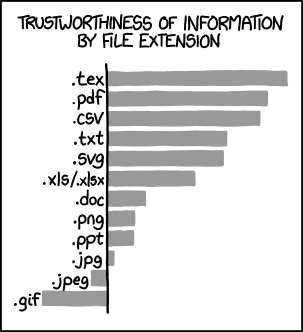
\includegraphics[width=0.4\textwidth]{images/file_extensions.png}
\end{figure}
{\textcolor{white}{\tiny\href{https://xkcd.com/1301/}{https://xkcd.com/1301/}}}
}